% Capítulo 2
\chapter{Metodologia}\label{cap:metodologia}

Este estudo adota uma abordagem aplicada, com o objetivo de gerar conhecimento prático e oferecer soluções na área de avaliação educacional em programação. A pesquisa combina métodos quantitativos e qualitativos para a coleta e análise dos dados, conforme sugerido por \parencite{Gil2017}, que ressalta a importância de abordagens abrangentes para investigações detalhadas orientadas para a prática. Como estratégia principal, foi escolhido o estudo de caso, uma vez que permite explorar situações reais com limites pouco definidos, mantendo a unidade do objeto de estudo e descrevendo seu contexto. Embora tenha sido realizada uma busca sucinta por referências teóricas, essa etapa seguiu um enfoque direcionado e seletivo, com o propósito de identificar trabalhos relevantes ao tema, configurando assim uma pesquisa na literatura, porém  de escopo reduzido, um levantamento teórico voltado à construção dos fundamentos necessário para o desenvolvimento da proposta que será discutida neste capítulo.

\section{Pesquisa de Trabalhos Relacionados}

A primeira etapa desta pesquisa consiste em explorar trabalhos recentes na literatura sobre a geração automática de questões de programação, a fim de conhecer o estado da arte e reunir a base teórica para o desenvolvimento deste estudo. Nesse processo, será realizada uma triagem com base em palavras-chave, selecionando os trabalhos por meio da análise dos títulos e resumos, seguida de uma leitura aprofundada dos trabalhos escolhidos. Essa abordagem permite identificar contribuições, desafios e lacunas relacionados à geração automática de questões de programação, fornecendo a base para responder à questão de pesquisa (\textbf{QP2}). 


\section{Desenvolvimento da Ferramenta}
Na segunda etapa, envolve a construção de um sistema capaz de executar os templates de questões de programação, gerando questões diversificadas e contextualizadas. Um mecanismo de combinação que facilita as combinações dos elementos das questões, e o uso do \gls{chatgpt} para recomendar diversos pontos de variação em cada ponto modificável do template. Após a apresentação da questão gerada e a submissão da resposta pelo aluno, o sistema, conectado à \gls{api} do \gls{chatgpt}, recebe a questão e a resposta submetida e, com base nessas informações e em um \textit{prompt} específico, gera um feedback detalhado, contribuindo para um processo de aprendizagem mais dinâmico. A Figura~\ref{fig:fluxo_desenvolvimento} apresenta um fluxograma com as principais etapas envolvidas no desenvolvimento da ferramenta, desde a definição dos requisitos até a entrega do feedback ao aluno:

\begin{figure}[ht]
	\centering
	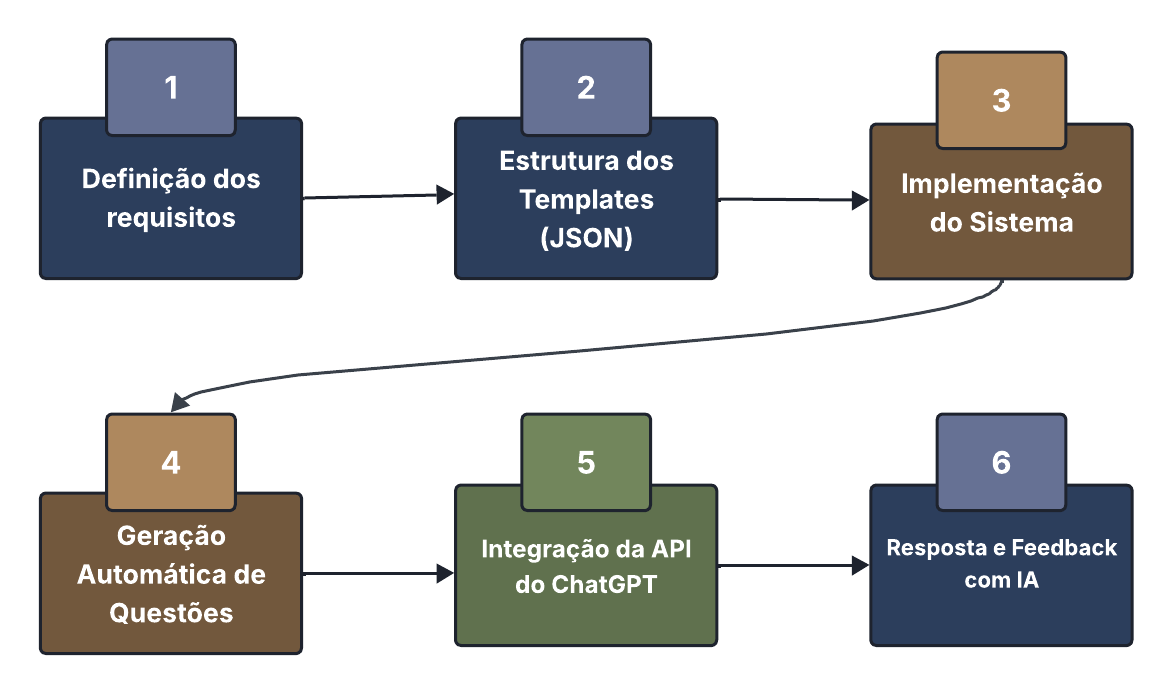
\includegraphics[width=12cm]{./imagens/capitulo2/fluxograma}
	\caption{Fluxograma : Etapas do desenvolvimento (Autoria própria, 2025)}
	\label{fig:fluxo_desenvolvimento}
\end{figure}

\subsection{Etapas do Desenvolvimento}
Com base no fluxo apresentado na figura \ref{fig:fluxo_desenvolvimento} , é possível detalhar cada uma das etapas que compõem o desenvolvimento da ferramenta. A seguir, temos os principais processos envolvidos, desde a concepção dos templates até a implementação técnica e o formato de estruturação dos dados utilizados no sistema.

\begin{enumerate}[label=\textbf{\arabic*)}]
    \item \textbf{Definição dos requisitos:} Identificação das necessidades funcionais da ferramenta, considerando os objetivos da geração automática de questões multicamadas.

    \item \textbf{Design dos templates JSON:} Criação de templates multicamadas utilizando o formato \gls{json}, escolhidos por sua leveza, eficiência e ampla aceitação em sistemas web \parencite{goyal2017, wang2011}. Esses templates estruturam elementos como enunciado, variáveis, contexto e nível de dificuldade.

    \item \textbf{Implementação do sistema:} Desenvolvimento da aplicação utilizando a linguagem Python e o framework Django. Essa escolha se justifica pela reutilização de componentes e separação clara de responsabilidades no sistema, como defendido por \parencite{rubio2017}.

    \item \textbf{Geração automática de questões:} A partir dos templates definidos, o sistema realiza combinações entre os componentes para gerar questões diversas e contextualizadas.

    \item \textbf{Integração com a API do ChatGPT:} A \gls{api} do \gls{chatgpt} é utilizada para sugerir variações nos pontos modificáveis dos templates e para processar as respostas submetidas, oferecendo feedback personalizado com base em \textit{prompts} específicos.

    \item \textbf{Resposta e feedback com IA:} Após o envio das respostas pelos estudantes, o sistema analisa as informações e retorna um feedback detalhado, promovendo um processo de aprendizagem mais eficaz e interativo.
\end{enumerate}


\section{Execução do Estudo de Caso}

Nesta seção, serão apresentados os principais aspectos do estudo de caso, que busca avaliar a efetividade dos templates, coletando dados qualitativos e quantitativos para analisar desempenho, clareza e relevância das questões geradas. 

\begin{enumerate}[label=\textbf{\alph*)}]
    \item \textbf{Planejamento e Metodologia:}  
    O estudo de caso será conduzido com o objetivo de avaliar a efetividade dos templates multicamadas e do sistema de geração automática de questões. A metodologia incluirá a aplicação prática dos templates e a coleta de dados qualitativos e quantitativos para análise de desempenho, dificuldade, clareza e relevância das questões geradas. 

    \item \textbf{Participantes do Estudo:}  
    Os participantes serão professores da área de computação, que lecionam disciplinas introdutórias de programação. Eles serão responsáveis por criar templates utilizando a ferramenta desenvolvida, com instruções específicas para estruturar pontos de variação nos modelos. As questões serão geradas a partir dos templates criados, abrangendo temas como entrada e saída, operadores lógicos, estruturas condicionais, laços de repetição e funções.

    \item \textbf{Aplicação dos Templates:}  
    Os professores participarão de atividades práticas de desenvolvimento de templates, explorando o funcionamento da ferramenta e contribuindo com a criação de novos modelos. As questões geradas pelos templates serão respondidas, permitindo aos participantes submeterem suas respostas e receberem feedback detalhado fornecido com o auxílio da Inteligência Artificial Generativa.

    \item \textbf{Coleta e Análise de Dados:}  A coleta de dados será realizada por meio da aplicação de questionários para avaliar a clareza e relevância das questões geradas com o intuito de identificar desafios, esforços, limitações e benefícios percebidos durante a criação e utilização dos templates. 
\end{enumerate}
    


\section{Resultados Esperados}

É esperado que a abordagem de geração automática de questões baseada em templates  proporcione benefícios significativos tanto para o processo de elaboração de questões quanto para a resolução das questões. Entre esses benefícios,  destaca-se a redução do esforço necessário para criar questões tradicionais, o aumento da geração de questões em escala, elaboração de questões contextualizadas e, por fim, a melhora do engajamento dos estudantes, impulsionada pela disponibilização de feedback imediato sobre suas respostas. Ao término do estudo de caso, será possível responder às questões de pesquisa relativas às vantagens da geração automática de questões (\textbf{QP1}), aos desafios inerentes à criação de templates (\textbf{QP2} e \textbf{QP3}). Assim, o estudo contribuirá para identificar limitações, oportunidades de melhorias e orientação para trabalhos futuros.



...



....


...



% Capítulo 2
\chapter{Metodologia}\label{cap:metodologia}

\noindent
\textbf{Ponto de ligação com o Capítulo 1.}  
No capítulo anterior apresentamos o problema de pesquisa, os objetivos e a motivação para automatizar a elaboração de questões de programação. A seguir descrevemos, de forma detalhada, a metodologia empregada para atingir tais objetivos.

Este estudo adota uma abordagem \textit{aplicada}, voltada à geração de conhecimento prático e à oferta de soluções para a avaliação educacional em programação. Combina métodos quantitativos e qualitativos de coleta e análise de dados, conforme sugerido por \textcite{Gil2017}, que destaca a importância de abordagens abrangentes em investigações orientadas para a prática.  

Como estratégia principal, foi escolhido o \textit{estudo de caso}, pois possibilita explorar situações reais com limites pouco definidos, preservando a unidade do objeto de estudo e descrevendo seu contexto. Embora tenha sido realizada apenas uma busca direcionada por referências teóricas, tal busca configurou—pela sistemática adotada—uma \textbf{revisão de literatura do tipo sistemática, porém de escopo reduzido}. Os resultados desse levantamento, com suas limitações, serão discutidos no \textbf{Capítulo 3}.

\section{Pesquisa de Trabalhos Relacionados}

A primeira etapa desta pesquisa consiste em mapear os trabalhos recentes sobre geração automática de questões de programação. A triagem será feita por palavras‑chave, análise de títulos e resumos, seguida de leitura aprofundada dos estudos selecionados. Esse processo permitirá identificar contribuições, desafios e lacunas — base para responder à questão de pesquisa \textbf{(QP2)}.

\section{Desenvolvimento da Ferramenta}

Na segunda etapa será construído um sistema capaz de executar templates multicamadas para gerar questões diversificadas e contextualizadas. Um mecanismo de combinação de elementos das questões — aliado a recursos de \gls{ia} generativa — recomendará variações em cada ponto modificável do template. Após a submissão da resposta pelo estudante, a IA fornecerá \textit{feedback} detalhado em tempo real, dinamizando a aprendizagem.


\subsection{Etapas do Desenvolvimento}
\begin{enumerate}[label=\textbf{\alph*)}]
    \item \textbf{Design dos templates}: criação de templates multicamadas que combinem enunciados, variáveis, contextos e níveis de dificuldade.
    \item \textbf{Auxílio da IA generativa}: recomendação de variações nos templates e fornecimento de \textit{feedback} imediato.
    \item \textbf{Implementação técnica}: uso de Python e Django\,—\,tecnologias livres, de alto desempenho e bem documentadas \parencite{rubio2017}.
    \item \textbf{Formato dos dados}: adoção de \gls{json}, por sua leveza e eficiência \parencite{goyal2017, wang2011}.
\end{enumerate}

\section{Execução do Estudo de Caso}

Nesta etapa avaliamos a efetividade dos templates por meio de dados qualitativos e quantitativos acerca de desempenho, clareza e relevância das questões.

\subsection{Planejamento e Metodologia}
Aplicação prática dos templates e coleta de dados sobre dificuldade, clareza e relevância.

\subsection{Participantes do Estudo}
Os participantes serão \textbf{professores de Computação} que:

\begin{itemize}
    \item lecione(m) ou tenha(m) lecionado disciplinas de \textit{Introdução à Programação};
    \item possuam \textbf{mínimo de 2 anos} de experiência docente (média esperada: 6 anos);
    \item atuem em instituições públicas ou privadas de ensino superior;
    \item concordem em criar templates com a ferramenta e responder ao questionário do Apêndice A.
\end{itemize}

\subsection{Aplicação dos Templates}
Os professores criarão templates, gerarão questões sobre entrada/saída, operadores lógicos, condicionais, laços e funções, responderão às questões e receberão \textit{feedback} automático.

\subsection{Coleta e Análise de Dados}
Dados serão coletados por:

\begin{itemize}
    \item \textbf{Questionário on‑line} (ver Apêndice A) para mensurar clareza, relevância e esforço percebido;
    \item \textbf{Logs} do sistema (tempo de elaboração, número de variações geradas, taxa de acerto dos estudantes);
    \item \textbf{Entrevistas semiestruturadas} para captar impressões qualitativas.
\end{itemize}

Análises estatísticas simples (médias, desvios‑padrão) e análise temática qualitativa serão combinadas para triangulação dos achados.

\section{Resultados Esperados}

Espera‑se reduzir esforço de criação de questões, aumentar a escala de itens e elevar o engajamento discente via \textit{feedback} imediato. O estudo permitirá responder às questões \textbf{QP1, QP2 e QP3}, identificar limitações e propor melhorias.

\bigskip
\noindent
\textbf{Ponto de ligação com o Capítulo 3.}  
O próximo capítulo descreve, em detalhe, a revisão sistemática concisa que embasa a presente metodologia, destacando as principais lacunas encontradas e justificando o foco nos templates multicamadas.
